\chapter{Time-dependent dynamical systems}
Our setup for this chapter will be of nonautonomous $n$-dimensional systems, i.e. the following
\begin{align}
	\dot{x}=f(x,t);\quad x \in \mathbb{R}^{n};\quad t \in \mathbb{R}.
\end{align}
Note that by adding a dimension to our phase space, we can make the system autonomous
\begin{align}
	X =
	\begin{pmatrix}
		x \\ t
	\end{pmatrix}\in \mathbb{R}^{n+1};
	\quad F(X) =
	\begin{pmatrix}
		f \\ 1
	\end{pmatrix}
	\implies
	\dot{X} = F(X).
\end{align}
\section{Nonautonomous linear systems}
For this section, consider
\begin{align}
	\dot{x} = A(t)x + b(t);\quad x \in \mathbb{R}^{n};\quad A(t)\in \mathbb{R}^{n\times n};\quad b(t) \in \mathbb{R}^{n}. \numberthis \label{eq6:star}
\end{align}
We separate \eqref{eq6:star} into two parts. The homogeneous part is
\begin{align}
	\dot{x} = A(t)x \numberthis \label{eq6:homo}.
\end{align}
For the homogeneous part we have the solution $x(t) = \Phi_{t_0}^{t}x_0$, with the fundamental matrix solution $\Phi$ with the property $\Phi_{t_0}^{t_0} = I \in \mathbb{R}^{n\times n}$. The general solution of \eqref{eq6:star} is the sum of the general solution of \eqref{eq6:homo} and a particular solution of \eqref{eq6:star}. We can find the particular solution by, for example, the variation of constants formula. We refer to \cite{Arnold} for the derivation.  
Thus we find the general solution to \eqref{eq6:star} to be
\begin{align}
	\boxed{
		x(t) = \Phi_{t_0}^{t} x_0 + \Phi_{t_0}^{t}\int_{t_0}^{t} \left( \Phi_{t_0}^{s}\right)^{-1}b(s) ds.
	}
\end{align}
Note that due to the group property of the flow map, the solution can be equivalently written as
\begin{align}
x(t) = \Phi_{t_0}^t x_0 + \int_{t_0}^t \Phi_s^t b(s) ds.
\end{align}
From here we can see that it is enough to understand the homogeneous part. The stability of $x=0$ in \eqref{eq6:homo} is equivalent to the stability of
	$x_p(t) = \Phi_{t_0}^{t}\int_{t_0}^{t} \left( \Phi_{t_0}^{s}\right)^{-1}b(s)ds$
in \eqref{eq6:star}.
Unfortunately the general solution to \eqref{eq6:homo} is unknown.

\section{Time-periodic nonlinear systems}
We now specify our system to be $T$-periodic, thus the evolution rule defined by $\dot{x}=A(t)x$ repeats itself with period $T$, i.e.
\begin{align}
	A(t+T) = A(t).
\end{align}
This implies
\begin{align}
	\Phi_{t_0}^{t_0 +T} = 	\Phi_{t_0+T}^{t_0 +2T} =\Phi_{t_0+2T}^{t_0 +3T} =\ldots =: P_{t_0},  
\end{align}
The operator $P_{t_0}$ is called the \emph{Poincaré map} (or time $T$ map) based at $t_0$. Thus we have
\begin{align}
x_0(t_0+nT) = \underbrace{P_{t_0} \ldots P_{t_0}}_{n  \textrm{ times} } = P_{t_0}^{n}x_0.
\end{align}
The $n$-th iterate of the Poincaré map is denoted by $P_{t_0}^{n}$.

Time being a periodic variable allows us to study the geometry in the extended phase space $\mathbb{R}^{n}\times S^{1}$ as depicted in Fig. \ref{fig:poinc_geom}.
\begin{figure}[h!]
	\centering
	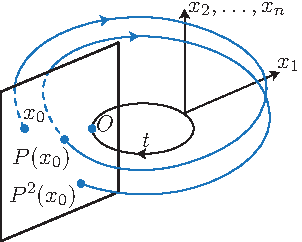
\includegraphics[width=0.6\textwidth]{figures/ch5/1poinc_geom.pdf}
	\caption{The map P records snapshots of the trajectory $x(t)$ taken at times $nT$. These snapshots are depicted along a single plane in the extended phase space. Due to periodicity, the extended phase space is made up as the product of the plane and the circle $S^1$. The snapshots shown are $Px_0 = x_1$ and $P^2 x_0 = x_2$.}
	\label{fig:poinc_geom}
\end{figure}
Importantly, the stability of $x=0$ can be studied as the stability of the $x=0$ fixed point of the map $P_{t_0}$. Label the eigenvalues of $P_{t_0}$ $\rho_1,\ldots,\rho_n\in\mathbb{C}$ these are called \emph{Floquet multipliers}. Since this is now a discrete dynamical system, we know how to assess the stability type of its fixed point. We have two cases
\begin{enumerate}
	\item If there exists an eigenvalue with $|\rho_i|>1$ for $P_{t_0}$ or there exists a repeated eigenvalue with $|\rho_j|=1$ for which the algebraic multiplicity is greater than the geometric multiplicity ($a>g$), then $x=0$ is unstable for \eqref{eq6:homo};
	\item Otherwise, if each eigenvalue of $P_{t_0}$ has magnitude strictly less than 1, i.e. $|\rho_j|<1$, then $x=0$ is asymptotically stable for \eqref{eq6:homo}.
\end{enumerate}

Floquet theory tells us that the following holds in general
\begin{align}
	\boxed{
		\Phi_{t_0}^{t} = {B(t)} e^{\Lambda(t-t_0)};\quad B(t+T) = B(t)\in \mathbb{R}^{n\times n};\quad \Lambda \in \mathbb{R}^{n\times n}  \textrm{ is constant} .
	}
\end{align}
\begin{definition}[Floquet exponents]
	The eigenvalues of $\Lambda$ are $\lambda_1,\ldots,\lambda_n\in \mathbb{C}$ and they are called \emph{Floquet exponents}. The previously defined Floquet multipliers are related to $\lambda_j$ as 
	\begin{align}
		\boxed{
			\rho_j = e^{\lambda_j T} = e^{(\alpha_j + i \beta_j)T}.
		}
	\end{align}
	Hence, $\lambda_j$ is well-defined only up to addition of $i2k\pi /T$ for $k \in \mathbb{Z}$. Therefore we have 
	\begin{align}
		|\rho_j| \underset{>}{\overset{<}{=}}1 \Leftrightarrow  \textrm{Re} \lambda _j \overset{<}{\underset{>}{=}} 0.	
	\end{align}
This is generally only numerically computable.	
\end{definition}

We now explore a sufficient criterion for instability of $x=0$. For this, recall Liouville's Theorem (Abel's Theorem)
\begin{align}
	\boxed{
		\det (\Phi_{t_0}^{t}) = \det(\Phi_{t_0}^{t_0})e^{\int_{t_0}^{t}  \textrm{Tr} \left[ A(s) \right] ds}.
	}
\end{align}
This holds true for any dynamical system $\dot{x}=A(t)x$ with aperiodic time-dependence.
\begin{proposition}[Sufficient criterion for instability]
	If we have $\int_{0}^{T}  \textrm{Tr} [A(s)]ds>0$ then $x=0$ is unstable for $\dot{x}=A(t)x$ with $A(t) = A(t+T)$
\end{proposition}
\begin{proof}
Apply Liouville's Theorem to our $T$-periodic system to find
\begin{align}
	\prod_{j=1}^{n} \rho_j = e^{\sum_{j=1}^{n} \lambda_j T} = \det(P_{t_0})	= \det(\Phi_{t_0}^{t_0+T}) = e^{\int_{t_0}^{t_0+T}  \textrm{Tr} \left[ A(s) \right] ds}.	
\end{align}
Now we can compare the arguments of the exponential functions to derive
\begin{align}
	\boxed{
		\sum_{j=1}^{n} \lambda _j = \frac{1}{T} \int_{0}^{T}  \textrm{Tr} \left[A(s) \right] ds.
	}
\end{align}
Therefore our claim holds due to the case differentiation for stability above.  Thus we can verify the stability without the numerical solution of \eqref{eq6:homo}.
\end{proof}
\begin{remark}[]
	The change of variables $x = P(t)y$, for some matrix $P(t)$ transforms the system \eqref{eq6:homo} into the form $\dot{y}=By$, an autonomous linear ODE.
	
	Carrying out the change of coorinates, we obtain that
	\begin{align}
		\dot{y} = P^{-1} (A(t)P - \dot{P})y.
	\end{align}
But
\begin{align}
	\frac{d}{dt}\left( P(t)e^{Bt}\right) = APe^{Bt} \implies \dot{P} + PB = AP.
\end{align}
Together this implies $\dot{y} = By$.
\end{remark}

\section{Averaging}
We will now attempt to study the mean evolution of oscillatory systems
\begin{align}
	\dot{x} = f(x,t);\quad x \in \mathbb{R}^{n};\quad f(x,t+T) = f(x,t).
\end{align}
In general the averaged system
\begin{align}
	\dot{y} = \frac{1}{T} \int_{0}^{T} f(y,t)dt	
\end{align}
does not capture the overall (mean) behavior of the system. This can be demonstrated in an example.
\begin{ex}[Averaging for a swing]
	Mechanically, we examine the stability of a pendulum with a periodically varying length as shown in Fig. \ref{fig:swing_drawing}.
	\begin{figure}[h!]
		\centering
		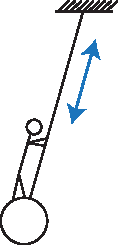
\includegraphics[width=0.15\textwidth]{figures/ch5/2swing_drawing.pdf}
		\caption{A swing (pendulum) with varying length and a mass $m$.}
		\label{fig:swing_drawing}
	\end{figure}
	The first order model for this system is
	\begin{align}
		\begin{dcases}
			\dot{x}_1 = x_2\\
			\dot{x}_2 = -\omega_0^2 (1+a(t))x_1
		\end{dcases}
		;\quad a(t) = a(t+T),\quad 0<|a|\ll 1.	
	\end{align}
Averaging these equations yields
\begin{align}
	\begin{dcases}
		\dot{x}_1 = x_2 \\
		\dot{x}_2 = -\omega_0^2(1+ \overline{a})x_1.
	\end{dcases}
\end{align}
Where $\overline{a}$ is the average of $a(t)$, a constant. The phase portrait of this is known, as it is just a standard pendulum, i.e. $x=0$ is stable. This means that the small forcing, when averaged, shouldn't move us from the stable position at $x=0$. But we know that by periodically swinging, we don't just stay stuck at the equilibrium point of the swing, but instead are able to reach larger amplitude oscillations. Therefore, averaging clearly does not work in this situation. 
\end{ex}

However, there are situations in which averaging does work.
\begin{ex}[Averaging in slowly varying periodic systems]
Slowly varying periodic systems are given by
\begin{align}
	\dot{x} = \varepsilon f(x, t, \varepsilon);\quad x \in \mathbb{R}^{n};\quad 0 \leq \varepsilon \ll 1;\quad f(x,t,\varepsilon) = f(x,t+T,\varepsilon).
\end{align}
Such systems are also called \emph{adiabatic} systems.
The averaged system in this case is
\begin{align}
	\dot{y} = \varepsilon \frac{1}{T} \int_{0}^{T} f(y,t,0)dt = \varepsilon \overline{f_0}(y).	
\end{align}
Here only the leading order terms with respect to $\varepsilon$ in the integrand were taken, as $\varepsilon \ll 0$. Now we transform our original equation into the averaged equation via a near-identity, periodic change of variables
\begin{align}
	x=y+\varepsilon w(y,t);\quad w(y,t) = w(y, t+T).
\end{align}
Plugging this transformation into our differential equation, we find
\begin{subequations}
\begin{align}
	\dot{x} &= \left[ I + \varepsilon D_{y}w\right]\dot{y} + \varepsilon \frac{\partial w}{\partial t} \\
	\dot{y} & = \underbrace{\left[ I + \varepsilon D_{y}w \right] ^{-1}}_{I - \varepsilon D_yw + \mathcal{O}(\varepsilon^2)}
	\left[\varepsilon  \underbrace{f(y+\varepsilon w(y,t),t,\varepsilon)}_{=\dot{x}} -\varepsilon \frac{\partial w}{\partial t} \right]\\ 
		&=\varepsilon \left[f(y,t,0) - \frac{\partial w}{\partial t}\right] + \mathcal{O}(\varepsilon)^2.
\end{align}
\end{subequations}
In the last equation we used the Taylor expansion. We cannot set $w(y,t) = \int_{0}^{t} f(y,s,0)ds$ as that would make $\omega $ aperiodic. Instead we separate $f$ into two parts, the average and the deviation, $f(y,t,0) = \overline{f}_0 (y) + \tilde{f}(y,t)$. Note that the deviation has mean 0, therefore we set $w(y,t) = \int_{0}^{t} \tilde{f}(y,s)ds$ which is periodic. Therefore we find $\dot{y} = \varepsilon \overline{f}_0(y) + \mathcal{O}(\varepsilon^2)$, noting here that the order 2 term is still $T$ periodic. 

This has given us that the original system is a $T$-periodic, $\mathcal{O}(\varepsilon^2)$ perturbation of the averaged system in the $y$ coordinates. 
\end{ex}

\begin{framed}
	\noindent
	\textbf{Averaging Principle} Solutions of the original equation starting $\mathcal{O}(\varepsilon)$ close to those of the averaged system, stay $\mathcal{O}(\varepsilon)$ close for times of $\mathcal{O}\left(\frac{1}{\varepsilon}\right)$ (very long).
\end{framed}

The averaging principle is depicted in Fig. \ref{fig:avg_principle}.
\begin{figure}[h!]
	\centering
	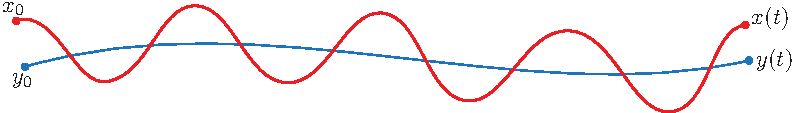
\includegraphics[width=0.99\textwidth]{figures/ch5/3avg_principle.pdf}
	\caption{For the starting point $x_0$ which is $\mathcal{O}(\varepsilon)$ close to $y_0$, the trajectories remain order $\varepsilon$ close, i.e. $x(t)$ is $\mathcal{O}(\varepsilon)$ close to $y(t)$, for $t \ll \frac{K}{\varepsilon}$.}
	\label{fig:avg_principle}
\end{figure}

This has implications for the Poincaré map of the original equation
\begin{align}
	P_{t_0}^{\varepsilon}:x_0 \mapsto x(t_0+T, x_0; \epsilon);\quad P_{t_0}^{\varepsilon} = P_{t_0}^{0} + \mathcal{O}(\epsilon) \implies \left( P_{t_0}^{\varepsilon}\right)^{n} = \left( P_{t_0}^{0}\right)^{n} + \mathcal{O}(\varepsilon).
\end{align}
This only holds if $n \leq \frac{1}{\varepsilon}$. The time $T$ map of the averaged system was denoted as $P_{t_0}^{0}$.

\begin{ex}[Averaged system with a saddle-type fixed point ]
	Consider a system whose Poincaré map $P_0$ has a hyperbolic fixed point $p_0$. By the persistence of hyperbolic fixed points, the perturbed Poincaré map $P_\varepsilon$ also has a hyperbolic fixed point $p_\varepsilon$ which is $\mathcal{O}(\varepsilon)$ close to $p_0$. Furthermore, the $\mathcal{C}^{1}$ manifolds $W^{U}_{ \textrm{loc} }(p_\varepsilon)$ and $W^{S}_{ \textrm{loc} }(p_{\varepsilon})$ are $\mathcal{O}(\varepsilon)$ close to their unperturbed counterparts. The unperturbed system and geometry of the perturbed system are shown in Fig. \ref{fig:avg_ex_2}.
	\begin{figure}[h!]
		\centering
		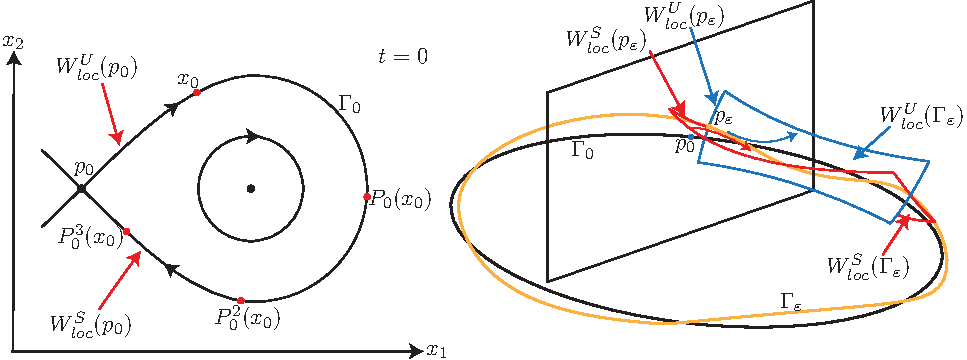
\includegraphics[width=0.99\textwidth]{figures/ch5/4avg_ex_2.pdf}
		%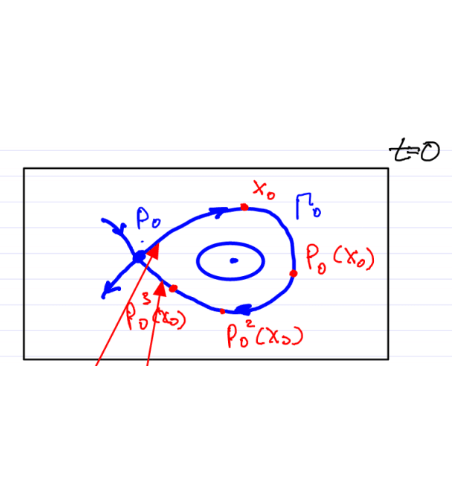
\includegraphics[width=0.37\textwidth]{figures/ch5/4avg_ex_2a.png}
		%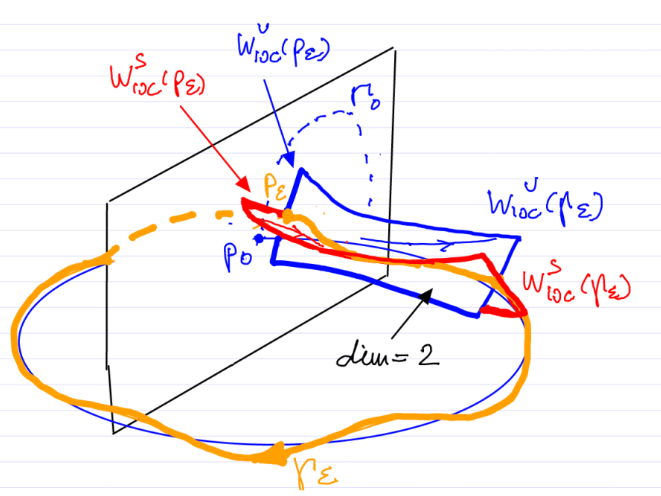
\includegraphics[width=0.6\textwidth]{figures/ch5/5avg_ex_2b.png}
		\caption{Left: The averaged system with the saddle type fixed point $p_0$. The upper arrow designates the local unstable manifold, and the lower arrow the local stable manifold. Right: The same in the extended phase space, time is represented by $S_1$ and runs clockwise. The hyperbolic limit cycle $\Gamma_\varepsilon$ is given by the yellow trajectory. Furthermore, the non-averaged local stable and unstable manifolds are drawn in red and blue respectively.}
		\label{fig:avg_ex_2}
	\end{figure}
	
\end{ex}
\begin{remark}[]
	We can show that fixed points persist for $P_\varepsilon$ as follows. First we take the flow map for the system $F_{t_0}^{t}(y_0;\varepsilon)$, then we use the Taylor expansion to find
	\begin{subequations}
	\begin{align}
		F_{t_0}^{t_0+T}(y_0; \varepsilon) &= F_{t_0}^{t_0+T}(y_0;0) + \varepsilon \frac{\partial}{\partial \varepsilon}F_{t_0}^{t_0 + T}(y_0;0)+ \mathcal{O}(\varepsilon^2) \\
						  &= y_0 + \varepsilon  \left.\frac{\partial y(t_0+T;t_0;\varepsilon)}{\partial \varepsilon} \right|_{\varepsilon=0} + \mathcal{O}(\varepsilon^2) \\
						  &= y_0 + \varepsilon \int_{t_0}^{t_0 +T} \overline{f}(y_0)dt + \mathcal{O}(\varepsilon^2) .
	\end{align}
\end{subequations}
	In the last equality we used that
	\begin{subequations}
	\begin{align}
		\left.\frac{ \partial y(t_0 + T; t_0, \varepsilon)}{\partial \varepsilon}\right|_{\varepsilon = 0} &=
			\left. \frac{\partial}{\partial \varepsilon} \int_{t_0}^{t_0+T} \dot{y}(s;t_0,\varepsilon)ds \right|_{\varepsilon=0} \\
		 &=\int_{t_0}^{t_0 +T} \left.\frac{\partial}{\partial \varepsilon } \left( \varepsilon \overline{f}(y(s)) + \mathcal{O}(\varepsilon^2)\right) \right|_{\varepsilon=0} ds \\
		 &= \int_{t_0}^{t_0 + T} \overline{f}(y_0) ds.
	\end{align}
\end{subequations}
	
From this we have
\begin{align}
	P_{\varepsilon}(y_0) - y_0 \Leftrightarrow y_0 +\varepsilon T \overline{f}(y_0) + \mathcal{O}(\varepsilon^2) - y_0=0 \Leftrightarrow  T \overline{f}(y_0) + \mathcal{O}(\varepsilon) = 0.
\end{align}
And now we can use the Implicit Function Theorem to conclude.
\end{remark}

\begin{ex}[Averaged system with a stable focus]
	Consider the averaged system with a stable focus around a fixed point $p_0 $. The transition to the perturbed system is shown in Fig. \ref{fig:avg_ex_3a}.
	\begin{figure}[h!]
		\centering
		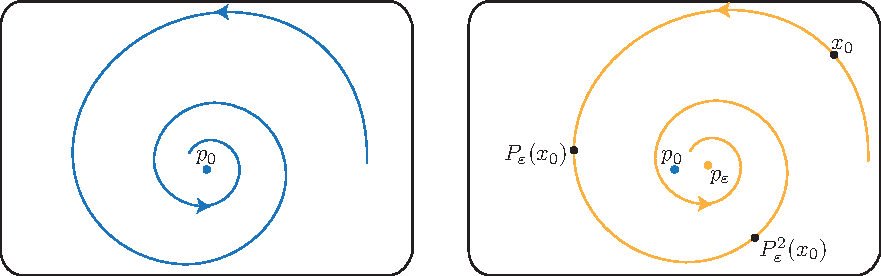
\includegraphics[width=0.99\textwidth]{figures/ch5/7avg_ex_3.pdf}
		%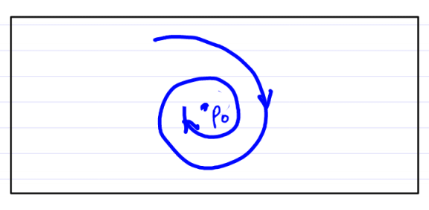
\includegraphics[width=0.4\textwidth]{figures/ch5/6avg_ex_3a.png}
		%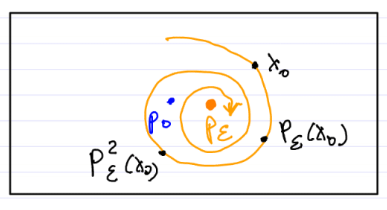
\includegraphics[width=0.4\textwidth]{figures/ch5/7avg_ex_3b.png}
		\caption{The stable focus around $p_0$ in the averaged system is preserved in the non-averaged system.}
		\label{fig:avg_ex_3a}
	\end{figure}
	
\end{ex}
\begin{ex}[Averaged system with a limit cycle]
	Consider the averaged system with a limit cycle $\Gamma_0$. The non-averaged system also has a stable limit cycle $\Gamma_\varepsilon$ with $ \textrm{dim }W^{S}(\Gamma_\varepsilon) =\mathbb{R}^{n+1} $ in extended phase space. Thus in the full system we have an attracting 2-dimensional invariant torus. The averaged and non-averaged system, along with this torus are shown in Fig. \ref{fig:avg_ex_3}.
	\begin{figure}[h!]
		\centering
		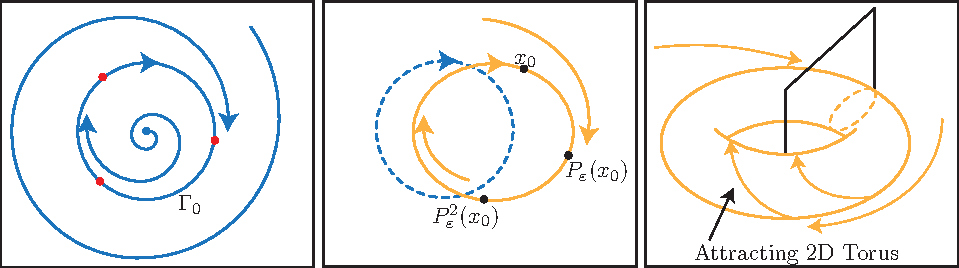
\includegraphics[width=0.99\textwidth]{figures/ch5/8avg_ex_4.pdf}
		%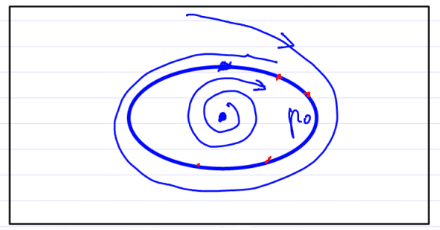
\includegraphics[width=0.34\textwidth]{figures/ch5/8avg_ex_4a.png}
		%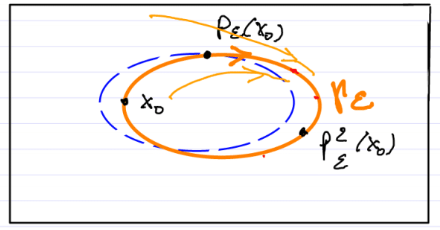
\includegraphics[width=0.34\textwidth]{figures/ch5/9avg_ex_4b.png}
		%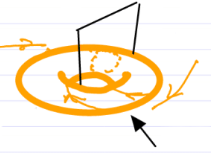
\includegraphics[width=0.3\textwidth]{figures/ch5/10avg_ex_4c.png}
		\caption{Left: The averaged system with the stable limit cycle $\Gamma_0$. Middle: The non-averaged system with the limit cycle $\Gamma_{\varepsilon}$. Right: The attracting 2-dimensional invariant torus (black arrow), trajectories can be seen as the thin yellow lines.}
		\label{fig:avg_ex_3}
	\end{figure}
	
\end{ex}

\begin{ex}[Weakly nonlinear oscillations]
	An important application of averaging is for weakly nonlinear oscillations. This is covered in-depth in \cite{GuckenheimerHolmes}. The system is given by
	\begin{align}
		\ddot{x} + \omega_0^2 x = \varepsilon f(x, \dot{x}, t) = \varepsilon f(x, \dot{x}, t+T);\quad T = 2\pi \omega .
	\end{align}
Averaging applies after a change of coordinates moving with the solutions of the $\varepsilon=0$ limit.	First transform the system to be a first-order ODE with $X= 
\begin{pmatrix}
	x \\ \dot{x}
\end{pmatrix}
$.
\begin{align}
	\dot{X} = AX + \varepsilon F(X,t); \quad A = 
	\begin{pmatrix}
		0 & 1 \\
		-\omega_0^2 & 0
	\end{pmatrix}
	;\quad
	F(X,t) = 
	\begin{pmatrix}
		0 \\ f(X_1, X_2, t)
	\end{pmatrix}
	\numberthis \label{eq6:1star}.
\end{align}
We cannot directly apply averaging to \eqref{eq6:1star}. Instead we introduce a coordinate change along the trajectories of the system. Let $\Phi(t;\omega_0)$ be the fundamental matrix of solutions. In fact, this is explicitly computable for the harmic oscillator as 
\begin{align}
	\Phi(t;\omega_0) =
	\begin{pmatrix}
		\cos(\omega_0 t) & -\sin(\omega_0 t) \\
		-\omega_0 \sin(\omega_0 t) & -\omega_0 \cos(\omega_0 t)
	\end{pmatrix}
	.
\end{align}
It can be checked that $\dot{\Phi} = A \Phi$. Thus we change coordinates with $X(t) = \Phi(t, \omega_0) Y(t)$. As $\Phi$ is invertible, we have $Y(t) = \Phi^{-1}(t, \omega_0) X(t)$ with the inverse
\begin{align}
	\Phi^{-1}(t,\omega_0) = 
	\begin{pmatrix}
		\cos(\omega_0 t) & -\frac{1}{\omega_0}\sin(\omega_0 t) \\
		-\sin(\omega_0 t) & - \frac{1}{\omega_0}\cos(\omega_0 t)
	\end{pmatrix}
	.
\end{align}
Now we substitute this transformation into the differential equation \eqref{eq6:1star} and use the fact that $\dot{\Phi} = A \Phi$ to find
 \begin{align}
	 \dot{\Phi}Y + \Phi \dot{Y} &= A\Phi Y + \varepsilon F(\Phi^{-1}Y, t)
	 \implies \dot{Y} = \varepsilon \Phi^{-1}F(\Phi Y, t). \numberthis \label{eq6:2star}
 \end{align}

 This appears to be in the required form for averaging, except the right hand side is not generally periodic, because $\Phi$ has frequency $\omega _0$, while the driving has frequency $\omega$. It is only periodic if $\omega= k \omega_0$ for $k \in \mathbb{Z}$, i.e. resonance of order $k$. Often it is important to analyze near-resonant oscillations, i.e. $\omega\approx k \omega_0$. Thus our expectation is to find an almost sinusoidal response of frequency $\frac{\omega }{k}$. Therefore we instead use the transformation  $\Phi(t; \frac{\omega }{k})$ and find
 \begin{align}
	 \dot{Y } = \Phi^{-1}\left[ A \Phi - \dot{\Phi}\right] Y + \varepsilon \Phi^{-1}F(\Phi Y, t). 	
 \end{align}
Now write $Y = 
\begin{pmatrix}
	u \\ v
\end{pmatrix}
$, and we find
\begin{align}
\begin{dcases}
	\dot{u} = -\frac{k}{\omega} \left[ \left( \frac{\omega^2 - k^2 \omega_0^2}{k^2}\right)x + \varepsilon f(x, \dot{x}, t) \right] \sin\left(\frac{\omega t}{k}\right) \\
	\dot{v} = -\frac{k}{\omega} \left[ \left( \frac{\omega^2 - k^2 \omega_0^2}{k^2}\right)x + \varepsilon f(x, \dot{x}, t) \right] \cos\left(\frac{\omega t}{k}\right)
\end{dcases}
\numberthis \label{eq6:uv}
\end{align}
Now we have that if $\omega^2 - k^2 \omega_0^2 = \mathcal{O}(\varepsilon)$, averaging applies to \eqref{eq6:uv}.

Next we consider a specific example, the Duffing oscillator
\begin{align}
	f(x, \dot{x}, t) = \beta \cos(\omega t) - \delta \dot{x} - \alpha x^3,
\end{align}
with $\omega_0^2-\omega^2 = \varepsilon \Omega$, i.e. a nearly order one resonance. The transformed system then takes the form
\begin{align}
	\begin{dcases}
		\dot{u} = \frac{\varepsilon}{\omega } [ &\Omega \left( u \cos(\omega t) - v \sin (\omega t)\right) - \omega \delta \left( u \sin(\omega t) + v \cos (\omega t)\right)  \\
							    &+\alpha \left(u \cos(\omega t) - v \sin (\omega t)\right) ^{3} - \beta \cos(\omega t)  ] \sin(\omega t)
\\
		\dot{v} = \frac{\varepsilon}{\omega } [ &\Omega \left( u \cos(\omega t) - v \sin (\omega t)\right) - \omega \delta \left( u \sin(\omega t) + v \cos (\omega t)\right)  \\
							    &+\alpha \left(u \cos(\omega t) - v \sin (\omega t)\right) ^{3} - \beta \cos(\omega t)  ] \cos(\omega t).
	\end{dcases}
\end{align}
Averaging over one period $T = \frac{2 \pi }{\omega }$ we find
\begin{align}
	\frac{1}{T} \int_{0}^{T} \sin(\omega t) \cos(\omega t) dt = \frac{1}{2T}\int_{0}^{T} \sin(2\omega t) dt = \left[ - \frac{\cos (2 \omega t)}{4 \omega T} \right]_{0}^{T} = 0,
\end{align}
and
\begin{align}
	\frac{1}{T}\int_{0}^{T} \sin^2 (\omega t) dt = \frac{1}{T} \int_{0}^{T} \frac{1-\cos(2\omega t)}{2} dt = \frac{1}{T} \left[ \frac{1}{2} - \frac{\sin (2 \omega t)}{2 \omega} \right]_{0}^{T} = \frac{1}{2}.
\end{align}
Using trigonometric identities then leads to the equation
\begin{align}
	\begin{dcases}
		\dot{u} = \frac{\varepsilon}{2 \omega }\left[ - \omega \delta u - \Omega v - \frac{3 \alpha }{4} ( u^2 + v^2) v\right] \\
		\dot{v} = \frac{\varepsilon}{2 \omega } \left[ \Omega u - \omega \delta v + \frac{3 \alpha}{4} (u^2 + v^2) u - \beta \right].
	\end{dcases}
\end{align}
This can be further simplified by using the polar coordinates $(r, \phi)$, i.e. 
\begin{align}
	\begin{pmatrix}
		u \\v
	\end{pmatrix}
	= 
	\begin{pmatrix}
		r \cos(\phi) \\
		r \sin (\phi)
	\end{pmatrix}
	\implies
	\begin{dcases}
		\dot{r} = \frac{\varepsilon}{2 \omega }\left[ - \omega \delta r - \beta \sin(\phi) \right] \\
		r \dot{\phi} = \frac{\varepsilon}{2 \omega } \left[ \Omega r + \frac{3 \alpha }{4 }r^3 - \beta \cos(\phi) \right].
	\end{dcases} \numberthis \label{eq6:2pound}
\end{align}
Next, recall that $x(t) = u(t) \cos(\omega t) - v(t) \sin(\omega t) = r(t)\cos(\omega t - \phi(t))$, i.e. we have slowly varying amplitude $r(t)$ and phase $\phi(t)$. The hyperbolic fixed points of \eqref{eq6:2pound} correspond to steady, almost sinusoidal response of the original system. We obtain the \emph{forced response curves} by fixing $\alpha,\ \beta,$ and $\delta$ and plotting the fixed point $(\overline{r}, \overline{\phi })$ of \eqref{eq6:2pound} as a function of the frequency parameter $\Omega $ (or $\frac{\omega }{\omega _0}$) as in Fig. \ref{fig:forced_response}.
\begin{figure}[h!]
	\centering
	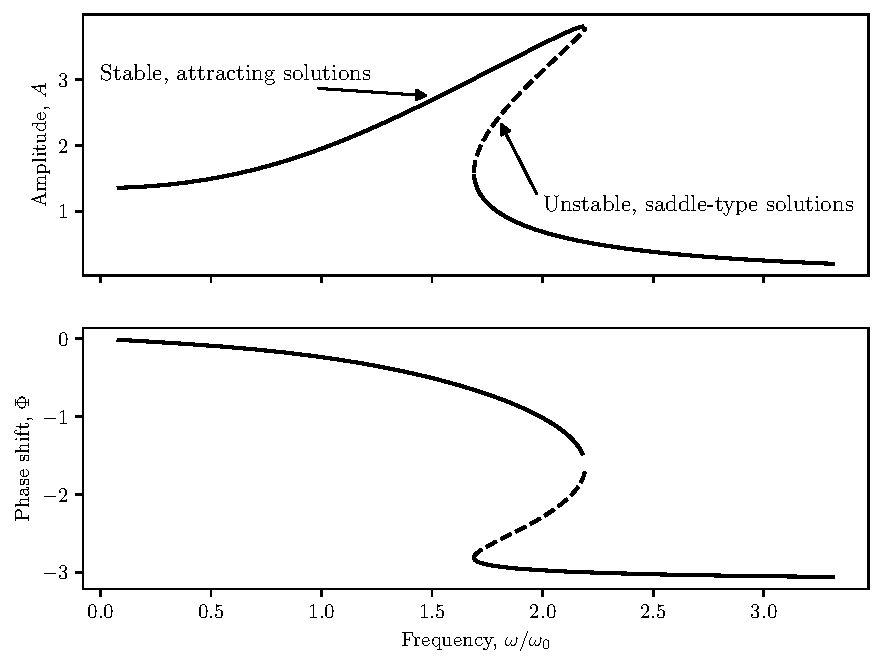
\includegraphics[width=0.5\textwidth]{figures/ch5/11forced_response.pdf}
	\caption{The forced response curve for the Duffing equation. The parameters are selected as $F_0 = 2, \omega_0=1, \alpha=0.35, \zeta = 0.12$. }
	\label{fig:forced_response}
\end{figure}

\end{ex}

\section{The Harmonic Balance Method}
Averaging and other perturbation techniques are often restrictive due to their small-parameter assumptions and result in cumbersome expressions limiting their application in high-dimensional systems. To avoid these constraints, the \emph{Harmonic Balance} method computes the Fourier series approximation of the periodic response and is formally applicable without the previous restrictions. Consider the setup 
\begin{align}
	\dot{x} = f(x,t) = f(x,t+T); \quad x \in \mathbb{R}^{n};\quad f \in \mathcal{C}^{r}_{x},\ r\geq 1,\ f \in \mathcal{C}^{0}_{t}. \numberthis \label{eq6:one}
\end{align}
Now we seek a $T$-periodic response via the Fourier series. 
\begin{remark}[]
	It is not immediately clear that a periodic response exists in a periodically forced multi-degree of freedom mechanical system. See for instance \cite{BreunningHaller} for more detail.
\end{remark}

	Assume \eqref{eq6:one} exhibits a $T$-periodic response, say $x_{p}(t) = x_{p}(t+T)$. Then it can be expressed as a convergent Fourier series
	\begin{align}
		x_p(t) = \sum_{k \in \mathbb{Z}}^{} \hat{x}_{k}e^{ik\omega t} = x_0 + \sum_{j \in \mathbb{N}}^{} c_j \cos(j \omega t) + s_j \sin(j \omega t).
	\end{align}
	Substituting this into \eqref{eq6:one} and using that $f$ is $T$-periodic (in both variables) and therefore admits a convergent Fourier series we find
	\begin{subequations}
	\begin{align}
		\frac{d}{dt}x_p(t)  &= 	f(x_p(t), t)\\
		\frac{d}{dt}\sum_{k \in \mathbb{Z}}^{} \hat{x}_k e^{ik \omega t}
				    &=	\sum_{k \in \mathbb{Z}}^{} \hat{f}_{k}(x_p(t), t) e^{i k \omega t} \\
		\sum_{k \in \mathbb{Z}}^{}  i k \omega \hat{x}_{k}e^{ik \omega t}	
				    &= \sum_{k \in \mathbb{Z}}^{} \hat{f}_{k} (x_p(t), t) e^{ik \omega t}.
	\end{align}
\end{subequations}
	Now we can compare coefficients at different harmonics to find
	\begin{align}
		ik \omega \hat{x}_{k} = \hat{f}_{k}(x_{p}(t), t) = \hat{f}_{k}\left( \sum_{j \in \mathbb{Z}}^{} \hat{x}_{j}e^{ij \omega t}, t \right) \quad \forall k.
	\end{align}
	These are algebraic equations which give a solution for each coefficient. In general they are coupled, with a noteworthy exception if $f$ is linear. However, there are infinitely many equations to solve, so in practice we only use a finite truncation of the Fourier series to approximate the response. 
	\begin{align}
		{x}_{H} = \sum_{k=-H}^{H} \hat{x}_{k}e^{ik \omega t}.
	\end{align}
	Now we instead solve $\dot{x}_H = f_{H}(x_{H}(t), t)$, leading to only $n(2H+1)$ equations.	
Recall a few basic results from Fourier Analysis.
\begin{theorem}[]
	For any $F\in \mathcal{C}^0$ which is $T$-periodic, the truncation $F_{H}(t) = \sum_{k=-H}^{H} \hat{F}_{k}e^{ik \omega t}$ converges uniformly to $F(t)$ as $H \to \infty $.
\end{theorem}
\begin{theorem}[Decay of Fourier coefficients]
	For $F\in \mathcal{C}^{r}$ which is $T$-periodic, the Fourier coefficients $\hat{F}_{k}$ decay at least as fast as $\frac{1}{|k|^{r+1}}$. For an analytic function $F\in \mathcal{C}^a$, the coefficients decay faster than any power of $k$, i. e. exponentially.
\end{theorem}
\begin{remark}[]
	Note that the decay estimate is asymptotic, hence it is generally unclear exactly where to truncate. However, the method seems to work well for many practical applications and produces fast results.
\end{remark}

We will now apply this method in a few examples.

\begin{ex}[Linear spring-mass-damper oscillator]
	Consider the following damped linear spring
	\begin{align}
		\ddot{x} + 2 \zeta \omega _0 \dot{x} + \omega _0^2 x = F(t) = F_0 \cos (\omega t). 
	\end{align}
	As only a single harmonic is sufficient to describe $F$, the harmonic coefficients are decoupled. By taking the Fourier series of $x$ and $F=\frac{1}{2}\left( F_0 e^{i \omega t} + F_0 e^{-i \omega t}\right)$ we compare coefficients
	\begin{subequations}
	\begin{align}
		k=1&: \quad - \omega ^2 \hat{x}_1 e^{i \omega t} + i 2 \zeta \omega_0 \omega \hat{x}_1 e^{i \omega t} + \omega_0^2 \hat{x}_1 e^{i \omega t} = F_0 e^{i \omega t};\\
		k=-1&: \quad  - \omega^2 \hat{x}_{-1}e^{-i\omega t} - i 2 \zeta \omega_0 \omega \hat{x}_{-1} e^{-i \omega t} + \omega_0^2 \hat{x}_{-1}e^{i \omega t} = F_0 e^{-i \omega  t}.
	\end{align}
\end{subequations}
We therefore calculate 
\begin{align}
	\hat{x}_1 = \frac{1}{2} \left( \frac{F_0}{\omega_0^2 - \omega ^2 + i 2 \zeta \omega_0 \omega }\right);
\quad	
	\hat{x}_{-1} = \frac{1}{2} \left( \frac{F_0}{\omega_0^2 - \omega ^2 - i 2 \zeta \omega_0 \omega }\right).
\end{align}
For all other values of $k$ $\hat{x}_{k}$ must equal zero. Now we can calculate the famous formula from linear vibration text books for the magnitude of the response
\begin{align}
	|x | =  \frac{F_0}{\omega_0^2\sqrt{\left( 1 - \left( \frac{\omega }{\omega_0}\right)^{2}\right)^2 + \left(2 \zeta \frac{\omega }{\omega_0}\right)^2  }}.
\end{align}

\end{ex}

\begin{ex}[Duffing Oscillator]
	Recall the Duffing oscillator
\begin{align}
	\ddot{x} + 2 \zeta \omega_0 \dot{x} + \omega_0^2  x + \alpha x^3 = F_0 \cos(\omega t).
\end{align}
We consider the Ansatz 
\begin{align}
	q_1(t) &= c_1 \cos(\omega t) + s_1 \sin(\omega t) \implies
	\ddot{q}_1 + 2 \zeta \omega_0 \dot{q}_1 + \omega_0^2 q_{1} + \alpha q_{1}^{3} = F_0 \cos(\omega t). 
\end{align}
Now calculate $q_1^3$ using multi-angle trigonometric identities
\begin{subequations}
 \begin{align}
	 q_1^{3} &= \left( c_1 \cos (\omega t) + s_1 \sin(\omega t)\right)^{3} \\
		 &= c_{1}^{3} \cos^{3}(\omega t) + 3 c_1^2 s_1 \cos^{2}(\omega t)\sin(\omega t) + 3 c_1 s_{1}^{2}\cos(\omega t) \sin^2(\omega t) +s_1^{3}\sin^{3}(\omega t) \\
		 &= \frac{1}{4} \left(3 c_1^3 + 3 c_1 s_1^2\right) \cos(\omega t) + \frac{1}{4} \left(c_1^3 - 3 c_1 s_1^2\right) \cos(3 \omega t) + \frac{1}{4} \left(3 c_1^2 s_1 + 3 s_1^3\right) \sin(\omega t) \\
		 &\quad + \frac{1}{4} \left(3 c_1^2 s_1 - s_1^3\right) \sin(3 \omega t). 
\end{align}
\end{subequations}
\end{ex}
Now we neglect the harmonics higher than 1 and balance the remaining
\begin{subequations}
\begin{align}
	0&=	\left[\left(\omega _0^2 - \omega^2\right) c_1 + 2 \zeta \omega_0 \omega s_1 + \frac{3}{4} \alpha \left(c_1^3 + c_1 s_1^2\right) - F_0 \right] \cos(\omega t)  \\
	 &\quad + \left[ \left( \omega_0^2 - \omega^2 \right) s_1 - 2 \zeta \omega_0 \omega c_1 + \frac{3}{4} \alpha \left(s_1^3 + c_1^2 s_1\right) \right] \sin(\omega t) +  \textrm{higher order harmonics}.  
\end{align}
\end{subequations}
Therefore we have two algebraic equations in $c_1$ and $s_1$. Using the polar coordinates $c_1 = A \cos(\phi)$ and $s_1 = A \sin(\phi)$ we find
\begin{subequations}
\begin{align}
	\left( \omega _0^2 - \omega ^2\right) A \cos(\phi) + 2 \zeta \omega_0 \omega A \sin (\phi) + \frac{3}{4} \alpha \left( A^3 \cos^3(\phi) + A^3 \cos(\phi) \sin^2(\phi) \right) &= F_0\\
	\left( \omega _0^2 - \omega ^2\right) A \sin(\phi) + 2 \zeta \omega_0 \omega A \cos (\phi) + \frac{3}{4} \alpha \left( A^3 \sin^3(\phi) + A^3 \sin(\phi) \cos^2(\phi) \right) &= 0.
\end{align}
\end{subequations}
Adding $\cos(\phi)$ times the first equation to $\sin(\phi)$ times the second we obtain
\begin{align}
	\left( \omega _0^2 - \omega^2 \right) A + \frac{3}{4} \alpha A^3 = F_0 \cos (\phi).
\end{align}
Similarly, adding $\sin(\phi)$ times the first equation to $\cos(\phi)$ times the second we obtain
\begin{align}
	2 \zeta \omega_0 \omega A = F_0 \sin (\phi).
\end{align}
We now take the sum of the squares of these two new equations, which yields
\begin{align}
	A^2 \left[ \left( \omega _0^2 - \omega ^2 + \frac{3}{4} \alpha A^2 \right) ^2 + 4 \zeta^2 \omega_0^2 \omega ^2 \right] = F_0^2.
\end{align}
This equation now allows us plot the amplitude $A$ versus the frequency $\omega$ as in Fig. \ref{fig:forced_response2}.
\begin{figure}[h!]
	\centering
	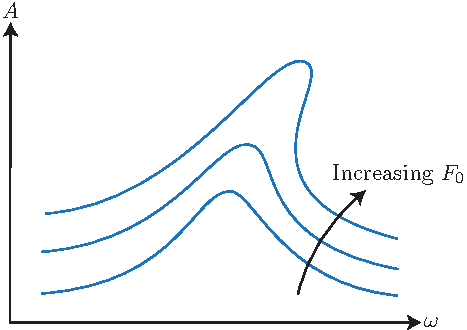
\includegraphics[width=0.6\textwidth]{figures/ch5/12forced_responce2.pdf}
	\caption{Forced response curves derived via harmonic balance for the Duffing oscillator.}
	\label{fig:forced_response2}
\end{figure}

Unfortunately, in contrast to averaging, harmonic balance by itself does not return any stability information. We can, however, compute the Floquet multipliers of the periodic orbit by directly solving the equation of variations. 

\begin{ex}[Unforced and undamped Duffing oscillator]
	For unforced systems harmonic balance can also be used to obtain internally parameterized periodic orbits. However, the expected period is a priori unknown. Consider the following
	\begin{align}
		 \ddot{x} + \omega _0^2 x + \alpha x^3 = 0.
	\end{align}
	Since the system in autonomous, the phase of the response is irrelevant. Thus the simplest Ansatz for a single harmonic response is
	\begin{align}
		x_1(t) = A \cos (\omega t),
	\end{align}
	for an unknown $\omega $. Applying the procedure as before and neglecting the higher harmonics we find
	\begin{align}
		\omega^2 = \omega_0 + \frac{3}{4} \alpha A^2.
	\end{align}
	For unforced, conservative, systems the frequency-amplitude relation gives the so-called \emph{backbone curve}, illustrated in Fig. \ref{fig:backbone}.
\begin{figure}[h!]
	\centering
	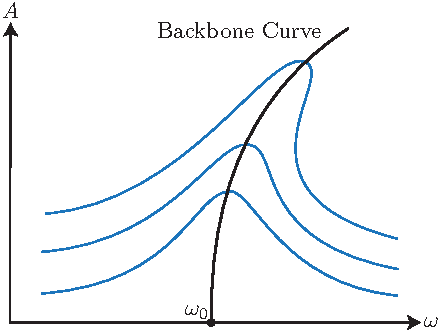
\includegraphics[width=0.6\textwidth]{figures/ch5/13backbone.pdf}
	\caption{The backbone curve for the unforced and undamped Duffing oscillator. Under small forcing and damping, the backbone curve has been observed to connect the forced response curves' peaks.}
	\label{fig:backbone}
\end{figure}
\end{ex}
